\documentclass{ieeeaccess}
\usepackage{cite}
\usepackage{amsmath,amssymb,amsfonts}
\usepackage{algorithmic}
\usepackage{graphicx}
\usepackage{textcomp}
\usepackage{array}
\usepackage{booktabs}
\usepackage{xcolor}
\usepackage{url}
\graphicspath{{figures/}{./}}

\setcounter{dbltopnumber}{4}
\renewcommand{\dbltopfraction}{0.9}
\renewcommand{\dblfloatpagefraction}{0.6}
\setcounter{totalnumber}{5}
\renewcommand{\topfraction}{0.9}
\renewcommand{\textfraction}{0.07}

\usepackage{bm}
\makeatletter
\AtBeginDocument{\DeclareMathVersion{bold}
\SetSymbolFont{operators}{bold}{T1}{times}{b}{n}
\SetSymbolFont{NewLetters}{bold}{T1}{times}{b}{it}
\SetMathAlphabet{\mathrm}{bold}{T1}{times}{b}{n}
\SetMathAlphabet{\mathit}{bold}{T1}{times}{b}{it}
\SetMathAlphabet{\mathbf}{bold}{T1}{times}{b}{n}
\SetMathAlphabet{\mathtt}{bold}{OT1}{pcr}{b}{n}
\SetSymbolFont{symbols}{bold}{OMS}{cmsy}{b}{n}
\renewcommand\boldmath{\@nomath\boldmath\mathversion{bold}}}
\makeatother

\newcommand{\vcite}[1]{\cite{#1}}

\newcommand{\nmath}[1]{\mbox{\mathversion{normal}$#1$}}

\begin{document}

\history{Resubmission of manuscript Access-2026-27906.}
\doi{10.1109/ACCESS.2026.DOI}

\title{Slice-Level Data Partitioning Inflates Pulmonary Nodule Classification Performance:
A Controlled Three-Arm Study}

\author{\uppercase{Nycolas Mariotto}\authorrefmark{1},
\uppercase{Jadson Gabriel Ferreira}\authorrefmark{1},
\uppercase{Jo\~ao Rafael Almeida de Andrade}\authorrefmark{1},
\uppercase{Jo\~ao Victor Carneiro Faria}\authorrefmark{1},
AND \uppercase{Allan Felipe Fattori Alves}\authorrefmark{1}}
\address[1]{Institute of Biosciences, S\~ao Paulo State University (UNESP), Botucatu, S\~ao Paulo 18618-689, Brazil}

\tfootnote{This work was supported by the Coordena\c{c}\~ao de Aperfei\c{c}oamento de Pessoal de N\'ivel Superior (CAPES), Brazil.}

\markboth
{Mariotto \headeretal: Data Partitioning in Pulmonary Nodule Classification}
{Mariotto \headeretal: Data Partitioning in Pulmonary Nodule Classification}

\corresp{Corresponding author: Allan Felipe Fattori Alves (e-mail: allan.alves@unesp.br).}

\begin{abstract}
Deep-learning studies on the LIDC-IDRI database routinely report pulmonary-nodule classification
accuracies above 95\% and AUCs above 0.99. Many partition data at the nodule or slice level, so
observations from one patient appear in both training and test folds. We test, \emph{by design},
whether the data-partition unit inflates reported performance: on a single cohort, with identical
labels, preprocessing, architecture, and training, we vary only the unit at which folds are formed
--- by patient, by nodule, or not at all --- and repeat over grouped cross-validation. Across $n=15$
matched folds (3 repeats $\times$ 5 folds) and three architectures spanning two model families, two
convolutional backbones and a vision transformer, random partitioning inflated slice-level
performance in every fold: the AUC gap was $+0.064$ (95\% CI $+0.031$ to $+0.097$) for DenseNet-121,
$+0.082$ ($+0.056$ to $+0.108$) for EfficientNet-B0 and $+0.074$ ($+0.036$ to $+0.112$) for
ViT-S/16, and calibration degraded in parallel (log-loss $+0.176$, $+0.315$ and $+0.221$; Brier
$+0.056$, $+0.080$ and $+0.067$). Aggregating predictions to the nodule level reproduced the effect
($+0.052$, $+0.060$ and $+0.057$). The gap was positive in 15 of 15 folds for every architecture
and survived re-scoring the arms on identical test rows. The nodule-grouped arm separates the
two routes a random split opens: under the assumption that they do not interact, we did not detect a
contribution from the patient route in any of the three architectures (interval permitting up to
$+0.059$ AUC), while within-nodule slice redundancy accounted for $81$--$98\%$ of the gap in
log-loss and Brier.
Partitioning below the nodule therefore inflates reported performance substantially, and grouping at
the nodule captured essentially all of the available protection in this cohort.
\end{abstract}

\begin{keywords}
Computed tomography, cross-validation, data leakage, data partitioning, deep learning, medical image
analysis, pulmonary nodules, reproducibility
\end{keywords}

\titlepgskip=-21pt

\maketitle

\section{Introduction}
\PARstart{L}{ung} cancer is the leading cause of cancer death worldwide, responsible for an estimated
1.8 million deaths in 2022~\vcite{bray2024}. Because prognosis depends strongly on the stage at
which the disease is found, low-dose CT screening of high-risk individuals is now widely
recommended: in the National Lung Screening Trial it lowered lung-cancer mortality by 20\% relative
to chest radiography~\vcite{aberle2011}. Screening and routine imaging in turn surface large numbers
of indeterminate pulmonary nodules, each of which must be characterized and managed according to its
estimated malignancy risk~\vcite{macmahon2017}. This triage burden has made automated malignancy
classification on CT one of the most active problems in medical image analysis, with the Lung Image
Database Consortium and Image Database Resource Initiative (LIDC-IDRI)~\vcite{armato2011} as its
standard benchmark.

Reported performance on this benchmark is strikingly high---accuracies above 95\% and areas under
the receiver-operating-characteristic curve (AUC) above 0.99 are common. Taken at face value, such
numbers would imply near-solved clinical decision support; but a classifier that appears 99\%
accurate while having learned to recognize \emph{patients} it has already seen, rather than
malignancy itself, would fail silently in deployment, where every patient is new. That such
performance has not translated into deployed tools motivates scrutiny of \emph{how} it is obtained.

One methodological choice recurs across this literature and is the subject of this paper: the unit
at which the data are divided into training and test sets. The choice matters here because
LIDC-IDRI is not a collection of independent images. It contains multiple nodules per patient and
multiple annotated slices per nodule, so when the division is performed at the nodule or the slice
level, slices belonging to the same patient can end up on both sides of the boundary. Those slices
share far more than the nodule they depict: they share anatomy, scanner, reconstruction kernel and
acquisition context. A model can therefore reach the right answer on a test image by recognizing the
patient it came from rather than by recognizing malignancy, which is a form of data leakage. It
inflates the reported test performance without improving the model, and it does so in a way that
cannot survive deployment, since every deployed patient is new.

The consequences of leakage are documented in adjacent medical-imaging domains. In brain-MRI
prediction, a reproducible re-evaluation found that leakage-free protocols reduce reported
performance~\vcite{wen2020}; in COVID-19 chest imaging, a systematic review found leakage among the
pitfalls that made published models unfit for clinical use, without quantifying its separate
contribution~\vcite{roberts2021}. Within
pulmonary-nodule classification the ingredients of the same problem are present, since correct
patient-level partitioning is used by only a minority of high-performing studies and is frequently
not reported at all (Section~\ref{sec:related}). What is missing is a comparable \emph{controlled}
test. The comparisons available so far set patient-level results against published numbers from
other groups, and those numbers differ in task, label definition, architecture and metric convention
as well as in partition unit, so a difference between them cannot be attributed to partitioning
alone. Attributing an effect to one variable requires holding the others fixed, which is what an
experiment does and a comparison across studies cannot.

\textbf{Gap.} No study on LIDC-IDRI has isolated the partition unit as the single manipulated
variable while holding cohort, labels, preprocessing, architecture, and training fixed, with
repeated cross-validation, uncertainty quantification, and paired significance testing.

\textbf{Contributions.} This paper makes three contributions. (i) It reports a controlled paired experiment in
which the partition unit is the only variable that changes, repeated over grouped cross-validation
so that every effect carries per-fold uncertainty and a paired significance test rather than a single
number. (ii) It decomposes \emph{where} the inflation appears, separating the ranking of cases (AUC)
from the calibration of the probabilities attached to them (log-loss and the Brier score), which
turns the result into mechanistic evidence about leakage rather than a bare performance difference.
(iii) It releases a pipeline that can be re-executed rather than merely described: the partition
indices are committed, the per-sample probabilities are retained, the evaluation code is published,
and automated gates make it impossible to introduce a divergence between configuration and code, or
to mix runs from different experiments, without the pipeline failing.

\section{Related work}
\label{sec:related}
\textbf{High-performance nodule classification on LIDC-IDRI.} LIDC-IDRI~\vcite{armato2011} is the
standard benchmark for pulmonary-nodule malignancy classification, and reported performance on it is
consistently high. Recent transformer models illustrate the trend: a multitask Swin Transformer
reaches a malignancy ROC-AUC of $0.985$~\vcite{jin2025}, and a compact ViT-Small/16 reaches $92.3\%$
accuracy on a $315$-patch LIDC-IDRI subset~\vcite{thakur2026}; convolutional models commonly report accuracies
in the low-to-high $90\%$s~\vcite{alshabi2019gated,procan2021,xiao2020ens}. We adopt ViT-Small/16,
one of the architectures this literature itself uses, because pure global attention is the furthest
departure from convolution available at this scale and therefore the sharpest test of whether the
partitioning effect is specific to convolutional inductive biases. A hierarchical-windowed
transformer such as Swin would be a weaker instrument for that question, since windowed local
attention is itself quasi-convolutional.

\textbf{Data partitioning and leakage.} To see why the partition unit deserves an experiment of its
own, it helps to know how the choice is currently made and reported. Much of this literature
partitions data below the patient level, and frequently does not state the partition unit at all.
We read the methods sections of a purposive sample of high-performance LIDC-IDRI malignancy
classifiers and recorded, for each, the partition unit it declares. Ten are cited here, each with the
verbatim sentence on which we classified it, so that every case in the tally can be checked rather
than taken on trust. Of those ten, three formed cross-validation folds by patient. Three split at the
\emph{nodule} level, three reported a $k$-fold split without specifying the unit, and one described
no split procedure at all. The sample is purposive rather than systematic, so these counts describe
the studies we read and are not an estimate of a field-wide rate; what they establish is that
partitioning below the patient, and not reporting the unit, are both common enough to find
immediately among the best-performing papers.

The nodule-level splits are often stated plainly, so there is no ambiguity about what was
done: one widely reused pipeline randomly divided its ``$406$ malignant and $442$ benign nodules
\ldots into $10$ exclusive partitions''~\vcite{alshabi2019gated} without grouping by patient, while
others randomly divide nodules into train and test~\vcite{contrastdiag2024} or split ``based on
nodule ID''~\vcite{lmlcc2025}. A second group is simply silent: these report only ``$k$-fold
cross-validation'' without saying whether images of the same patient were kept together~\vcite{alshabi2019lg,procan2021,xiao2020ens}, and one gives per-set counts under a heading of data
``splitting'' with no description of the procedure at all~\vcite{attnpyramid2024}. This is not a new
observation, since a prior case study reached the same conclusion, that such studies ``rarely provide
the exact details about \ldots the sample selection process''~\vcite{pitfalls2021}.

The consequence follows from the structure of the dataset. Because LIDC-IDRI contains multiple
nodules per patient and multiple annotated slices per nodule, any of the choices above can place
images of one patient on both sides of the train/test boundary, which is a textbook instance of
\emph{data leakage} --- ``the introduction of information about the \ldots target that should not be
legitimately available''~\vcite{kaufman2012}. That said, the practice is not uniform: some studies do
partition by patient and say so, confirming ``no shared patients between the two \ldots sets''~\vcite{mcn2020}, adopting a patient-level cross-validation split~\vcite{cmixnet2019}, or reporting a
patient-level stratified split~\vcite{mase2025}. Our
point is therefore about consistency rather than universal error. Since a generalization claim is a
claim about unseen \emph{patients}, the patient is the unit at which folds should be formed, and
neither the nodule nor the slice will serve. We emphasize that this sample is purposive and
non-systematic, assembled to characterize how the partition unit is reported rather than to estimate
a prevalence; two further papers were paywalled and are not counted.

\textbf{Leakage audits in medical imaging.} Systematic audits in adjacent domains have quantified the
consequences. In Alzheimer's-disease classification from brain MRI, a reproducible-evaluation study
found that a large fraction of surveyed convolutional studies exhibited evident or unclear data
leakage, and that a leakage-free protocol produced substantially lower, more realistic performance~\vcite{wen2020}. In COVID-19 imaging, a review of models built on chest radiographs and CT concluded
that none was of clinical use, in large part because of data-handling pitfalls including leakage~\vcite{roberts2021}. These audits establish both the phenomenon and the method --- a controlled,
leakage-free re-evaluation; to our knowledge, the present study is the first to apply a controlled
\emph{paired} experiment to the nodule-partitioning question on LIDC-IDRI.

\textbf{Evidence from proper partitioning.} The one comparator that explicitly enforces scan-level
partitioning, the LNDb challenge~\vcite{pedrosa2021}, which withholds whole scans for testing,
reports performance in the realistic range rather than the $95$--$99\%$ common under nodule- or
slice-level splits. This is consistent with the hypothesis that the gap is attributable to the
partition unit rather than to architecture, preprocessing, or class definition --- the hypothesis the
present controlled experiment isolates and tests.

\section{Methods}

\subsection{Dataset, cohort, and patient grouping}
We use LIDC-IDRI~\vcite{armato2011} (1{,}018 CT series from 1{,}010 patients) via the \texttt{pylidc}
library~\vcite{hancock2016}. Each nodule was read by up to four radiologists; we cluster the
per-radiologist annotations into physical nodules with pylidc's default consensus clustering.

\textbf{Counting (annotation vs.\ nodule).} These two units are reported separately and never
conflated, addressing a specific ambiguity in the prior version. An \emph{annotation} is one
radiologist's reading of a $\geq 3$\,mm nodule (one malignancy score and its contours); a
\emph{nodule} is the physical lesion (a cluster of 1--4 annotations). In LIDC-IDRI this yields
6{,}859 $\geq 3$\,mm annotations that cluster into 2{,}651 physical nodules. Applying the median
label rule (below) leaves 1{,}695 binary-labeled nodules; 956 nodules with a median malignancy of
exactly 3 are excluded as indeterminate. The labeling and grouping unit is always the nodule.

\textbf{Cohort.} The principal cohort keeps every labeled nodule that at least one radiologist
annotated, an inclusive criterion chosen so that the cohort is comparable to the literature this
study audits rather than quietly cleaner than it. That gives 11{,}026 slice-samples (5{,}504
malignant / 5{,}522 benign) across 740 patients at the slice level, and 1{,}695 nodules (545
malignant / 1{,}150 benign) at the nodule level. The count of 740 patients is smaller than
LIDC-IDRI's 1{,}010 because it includes only those contributing at least one binary-labeled nodule;
the remaining 270 have only indeterminate nodules, whose median malignancy score is exactly 3, or
nodules below the size criterion, so they enter no arm of the experiment. Separately, a
high-agreement cohort restricted to nodules read by at least three annotators (6{,}973 slices / 879
nodules / 535 patients) is reported as a sensitivity analysis, to test whether label noise changes
the conclusions.
One property of the cohort matters more than the others for what follows: the number of slices
contributed by a patient ranges from 1 to 97, with a median of 11. Because a patient therefore
supplies many correlated images rather than a single independent observation, the unit at which folds
are formed is not a cosmetic choice, and this is what motivates grouping by patient.

\textbf{Acquisition characteristics.} Table~\ref{tab:cohort} summarizes the cohort and the
acquisition parameters of its 748 series, read from the DICOM headers. The cohort is acquired
heterogeneously --- four manufacturers, 18 distinct reconstruction kernels, 11 distinct slice
thicknesses, and tube currents spanning $28$--$582$\,mA --- while being homogeneous in tube voltage
(120\,kVp in the interquartile range). We report this because acquisition context is the channel
through which images of one patient could be recognized as belonging to that patient; documenting its
heterogeneity establishes that the channel is available in this cohort, which is a separate question
from whether a model exploits it.

\begin{table*}[t]
\centering
\caption{Cohort and acquisition summary. Acquisition parameters are read from one DICOM header per
series (748 series, 740 patients); continuous values are median [IQR] (range).}
\label{tab:cohort}
\small
\begin{tabular}{ll}
\hline
\multicolumn{2}{l}{\emph{Cohort (principal)}}\\
Patients & 740 \\
Nodules (binary-labeled) & 1{,}695 (545 malignant / 1{,}150 benign) \\
Slice samples & 11{,}026 (5{,}504 / 5{,}522) \\
Slices per patient & 11 [5--20] (1--97) \\
Nodules per patient & 2 [1--3] (1--14) \\
Nodule diameter (mm) & 8.1 [6.1--12.8] (2.6--49.9) \\
\hline
\multicolumn{2}{l}{\emph{Acquisition}}\\
Manufacturer & GE 61.9\%, Siemens 22.1\%, Philips 8.8\%, Toshiba 7.2\% \\
Reconstruction kernel & 18 distinct; STANDARD 38.8\%, BONE 15.4\%, B30f 10.2\% \\
Slice thickness (mm) & 2.00 [1.25--2.50] (0.60--5.00), 11 distinct \\
In-plane spacing (mm) & 0.70 [0.63--0.74] (0.46--0.98) \\
Tube voltage (kVp) & 120 [120--120] (120--140) \\
Tube current (mA) & 241.5 [80--320] (28--582) \\
\hline
\end{tabular}
\end{table*}

\textbf{Patient grouping.} The correct unit for a generalization claim is the \emph{patient}: every
image from a patient must lie entirely within one fold. That is how the reference condition of this
experiment is built: its folds are formed by grouping on patient identity, and we assert \emph{and
export} that no patient identifier appears in more than one of its train/validation/test partitions.
The other two conditions deliberately break that rule, which is the manipulation under study; each is
defined in Section~\ref{sec:design} and its realized leakage is measured rather than assumed. The assertion runs at split
time and is re-verified on the committed indices (Section~\ref{sec:repro}); we measured zero
patient overlap across train/test/validation in every patient-arm fold.

\subsection{Label definition}
Malignancy is binarized from the radiologists' 1--5 scores using the median across annotators:
scores 4--5 are malignant, 1--2 benign, and score-3 (indeterminate) nodules are excluded. This
follows established practice and keeps the label identical across all partitioning arms so it
cannot confound the contrast.

\subsection{Preprocessing}
Because each LIDC nodule carries up to four independent manual segmentations, the first step is to
reduce them to one. For each nodule we form its region of interest from the 50\% consensus mask, that
is, the voxels agreed by at least half of the radiologists who annotated that nodule. This follows
the ``$50\%$ rule'' introduced for building a single reference segmentation from the multiple manual
segmentations of a LIDC nodule~\vcite{kubota2011}, and it is computed with the \texttt{consensus}
routine of the \texttt{pylidc} library at its default agreement level~\vcite{hancock2016}, so the
step is reproducible rather than bespoke.

From that mask we take the in-plane bounding box, pad it by $8$\,mm so that the immediate
perinodular context is retained, and crop it from \emph{every axial slice the nodule spans}. Each
cropped slice becomes one network input, and is prepared as follows: the CT window is clipped to
$[-1000,400]$ HU, which spans air to bone and prevents extreme values elsewhere in the body from
compressing the range of interest, then rescaled to $[0,1]$, squared by center-padding so that the
aspect ratio is preserved, resized to $256\times256$, and replicated to three channels because the
ImageNet-pretrained backbones expect a three-channel input.

A nodule spanning $s$ slices therefore contributes $s$ slice-samples, 11{,}026 in total at a mean of
$6.5$ per nodule, and this is why the slice- and nodule-level counts differ so much: the nodule-level
cohort collapses each nodule to a single representative slice, its largest cross-section.
Preprocessing is \emph{identical} across all arms, which is what prevents it from explaining any
difference between them. We did not include image enhancement (for example CLAHE) as an experimental
factor, because adding it would enlarge the grid without bearing on the partition-unit question this
study isolates. The trade-off is worth naming rather than merely deferring: contrast enhancement
could plausibly raise absolute performance, and it could equally sharpen the acquisition-specific
texture that makes images of one patient recognisable as belonging together --- which would act on
the very route we are trying to measure. Applying it identically in all arms, as we do with the rest
of preprocessing, keeps it from explaining any difference between them, but it also means we cannot
say which of those two effects would dominate. We measure neither, and claim neither.

\subsection{The controlled paired design}\label{sec:design}

\begin{figure*}[t]
  \centering
  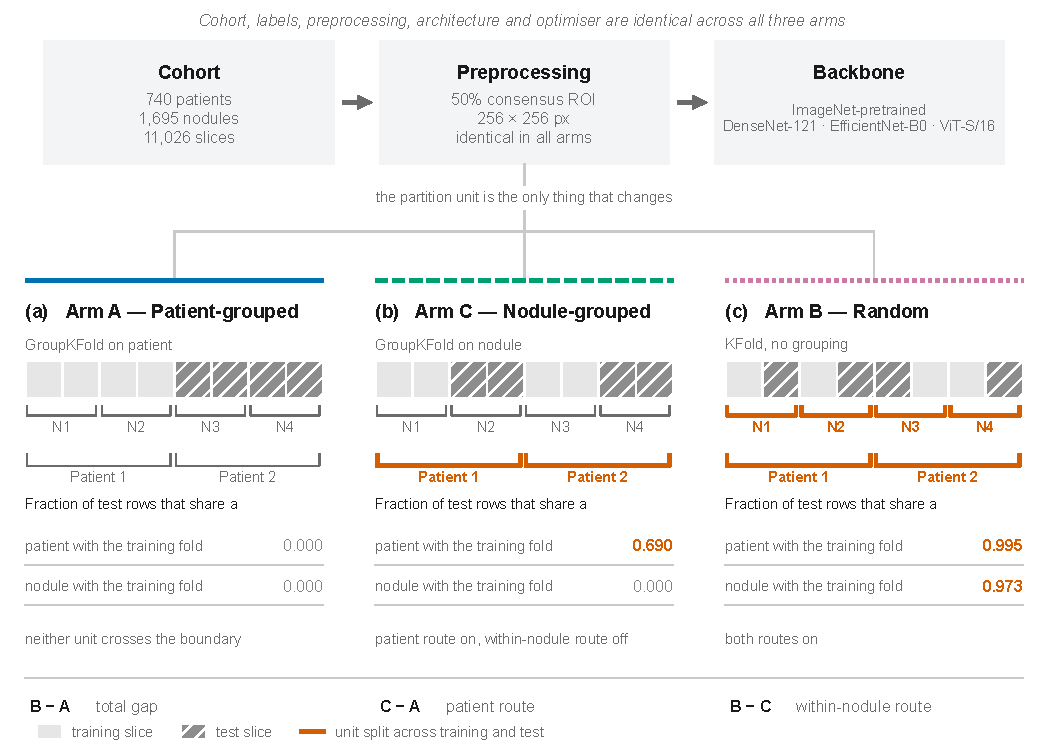
\includegraphics[width=\textwidth]{fig1_design.pdf}
  \caption{The controlled three-arm design. A single shared pipeline---identical cohort,
  preprocessing, and backbone---feeds three arms that differ \emph{only} in the unit at which folds
  are formed. Each arm's strip is a schematic of eight slices, two nodules from each of two
  patients, bracketed once by nodule and once by patient; a heavier vermillion bracket marks a unit
  that is split across training and test. Each arm reports the fraction of test rows that share a
  patient with the training fold --- the patient-leakage rate $L_{\mathrm{pat}}$ --- and the
  fraction that share a nodule, $L_{\mathrm{nod}}$. (a)~Arm~A groups by
  patient, so neither unit is split ($L_{\mathrm{pat}}=0.000$). (b)~Arm~C groups by nodule: every
  nodule stays whole ($L_{\mathrm{nod}}=0.000$) while a patient's nodules may fall on both sides
  ($L_{\mathrm{pat}}=0.690$), which leaves the patient route active at full sample density and
  switches the within-nodule route off. (c)~Arm~B assigns slices at random, so both units are split
  ($L_{\mathrm{pat}}=0.995$, $L_{\mathrm{nod}}=0.973$). Comparing the three arms decomposes the
  total gap into the two routes, using the same contrasts as Table~\ref{tab:routes}. Cohort counts
  and leakage rates are read from the released artifacts at render time and exported alongside the
  figure; no performance value is depicted.}
  \label{fig:design}
\end{figure*}

The experiment is a matched comparison of three arms that differ \emph{only} in the unit at which
folds are formed (Fig.~\ref{fig:design}). In arm~A (\emph{patient}) folds are formed by grouped
cross-validation on patient identity. In arm~B (\emph{random}) folds are formed by shuffling the
same samples, ignoring both nodule and patient. Arm~C (\emph{nodule}) is the intermediate condition:
folds are grouped by nodule, so every slice of a nodule stays on one side, but nodules are assigned
independently of the patient, so a patient's other nodules may fall across the boundary.
\textbf{Only the partition unit differs}---cohort, labels, preprocessing, architecture, optimiser,
schedule, and evaluation set size are held fixed. The design is repeated over $R=3$ repeats
$\times$ $K=5$ folds, giving $n=15$ matched folds per comparison, and the A-versus-B contrast is run
on both the slice and the nodule granularity (a $2\times2$ of partition-unit $\times$ sample-unit).
The leakage-advantage gap is reported per (architecture, sample-unit).

\textbf{Why the third arm.} Arms A and B differ in two ways at once, because a random split places
both \emph{slices of the same nodule} and \emph{nodules of the same patient} on opposite sides of the
boundary. The A-versus-B gap is therefore the combined effect of two routes and cannot say which one
produces it. Arm~C separates them: it eliminates the within-nodule route while leaving the
patient route active. Measured on the generated indices, the fraction of test samples whose patient
also appears in training is $0.000$ in arm~A, $0.995$ in arm~B and $0.690$ in arm~C, while the
fraction whose \emph{nodule} appears in training is $0.000$, $0.973$ and $0.000$ respectively.
Critically, arm~C retains nearly the reference arm's sample density ($12.4$ training slices per patient, against $14.9$ in
arm~A), so a null result for the patient route cannot be dismissed as too few samples per patient to
learn a patient-specific signature --- which is the objection that the nodule-\emph{sample-unit}
condition, at $1.9$ slices per patient, could not answer.

\textbf{Matched-rows control.} Because the arms have different test sets by construction, a gap
between them could in principle reflect test-set composition rather than leakage. We therefore also
re-score every pair of arms on the \emph{identical} rows --- the nodules and slices present in both
arms' test folds for that repeat and fold --- which holds composition, prevalence, size and
aggregation depth fixed and leaves only the trained model differing. Both the unmatched and the
matched gap are reported.

A central property of this matched design is that any factor shared identically by the arms
cancels in the arm-to-arm difference. In particular, the ImageNet-pretrained initialization, the
preprocessing, and the architecture are common to all arms; they may raise or lower the absolute
performance of each, but they cannot create a difference between them and therefore cannot bias the
reported gap. This is a substantive advantage over a single-number study, whose absolute metric
would inherit any such shared bias --- including any hidden overlap between a pretrained model's
(often undisclosed) training data and the evaluation set. Our claims are consequently stated as the
gap, not as absolute performance.

\subsection{Formalizing the leakage}
Let the dataset be $\mathcal{D}=\{(x_i,y_i,p_i,n_i)\}_{i=1}^{N}$, where $x_i$ is a slice, $y_i\in\{0,1\}$
its malignancy label, $p_i$ its patient and $n_i$ its nodule. A partition is a map
$\pi:\{1,\dots,N\}\to\{\mathrm{train},\mathrm{val},\mathrm{test}\}$. The arms differ \emph{only}
in $\pi$. The patient-grouped arm~A uses a $\pi_A$ that is constant on patients,
$p_i=p_j \Rightarrow \pi_A(i)=\pi_A(j)$, so the test set is patient-disjoint from train:
$\{p_i:\pi_A(i)=\mathrm{test}\}\cap\{p_i:\pi_A(i)=\mathrm{train}\}=\varnothing$. The random arm~B
assigns samples independently of $p_i$, so patients may straddle the boundary. The nodule-grouped
arm~C uses a $\pi_C$ that is constant on nodules but not on patients,
$n_i=n_j \Rightarrow \pi_C(i)=\pi_C(j)$ while $p_i=p_j \not\Rightarrow \pi_C(i)=\pi_C(j)$.

Define the patient-leakage rate of a partition as
\begin{equation}
L(\pi)=\frac{\bigl|\{i:\pi(i)=\mathrm{test},\ p_i\in\mathcal{P}_{\mathrm{train}}(\pi)\}\bigr|}
{\bigl|\{i:\pi(i)=\mathrm{test}\}\bigr|},
\end{equation}
where $\mathcal{P}_{\mathrm{train}}(\pi)=\{p_j:\pi(j)=\mathrm{train}\}$ is the set of patients
represented in the training partition.
By construction $L(\pi_A)=0$; empirically $L(\pi_B)\approx0.99$. For a metric $M$, the
leakage-advantage gap is $\Delta_M=M(\pi_B)-M(\pi_A)$ (sign reversed for log-loss/Brier). Because the
two arms are identical in cohort, labels, preprocessing, architecture and training and differ only
in $\pi$, $\Delta_M$ is attributable to the partition unit alone. For metrics that are means of
per-sample scores (log-loss, Brier, accuracy) this holds in the strong algebraic sense: if
$M(\pi)=g(\pi)+c$ with $c$ the shared component, then $\Delta_M=g(\pi_B)-g(\pi_A)$ is independent of
$c$. For rank metrics such as AUC, which are not additively separable across samples, the isolation
follows from the controlled comparison itself rather than from such a decomposition.

Slice-level leakage decomposes into two routes (which may overlap for a slice whose nodule and
whose patient are both represented in training),
\begin{equation}
\begin{aligned}
\{i\in\mathrm{test}&:p_i\in\mathcal{P}_{\mathrm{train}}\}=\\[2pt]
&\underbrace{\{i:\exists\,j\in\mathrm{train},\,n_i=n_j\}}_{\text{within-nodule redundancy}}\ \cup\\[2pt]
&\underbrace{\{i:\exists\,j\in\mathrm{train},\,p_i=p_j,\,n_i\neq n_j\}}_{\text{cross-nodule, same patient}},
\end{aligned}
\end{equation}
Arm~C is constructed to switch off the first term while leaving the second: $\pi_C$ is constant on
nodules, so no test slice shares its nodule with training, yet nodules are assigned independently of
the patient, so the second term remains populated ($L(\pi_C)=0.690$ measured). The three arms
therefore give $\Delta_M(B,A)$ for the combined effect, $\Delta_M(C,A)$ for the patient route alone,
and $\Delta_M(B,C)$ for the within-nodule route alone.

Two cautions govern how those three quantities may be read, and we state them before using them.
First, the identity $[M(C)-M(A)]+[M(B)-M(C)]=M(B)-M(A)$ is a telescoping sum and holds for any
metric; it is not evidence about a metric's structure. What does require structure is
\emph{attribution} --- reading $\Delta_M(C,A)$ as the share of the total produced by one route
requires the metric to decompose over the samples that route acts on. Log-loss, Brier and accuracy
are means of per-sample scores and do; AUC is a rank statistic over pairs and does not, so for AUC we
report the three gaps side by side and make no attribution claim. Second, the three arms are
separately trained models, not one model scored three ways, so describing the parts as routes assumes
the two do not interact --- that removing within-nodule redundancy does not change how the patient
route operates. Three arms cannot test that assumption, and every statement we make from this
decomposition carries it explicitly.

Note that aggregating predictions to the nodule level is a different operation and does \emph{not}
switch off the first term: it changes the unit at which predictions are scored, while the model has
still been trained with slices of one nodule on both sides of the boundary. Nodule-level aggregation
and nodule-level \emph{partitioning} are therefore distinct, and we keep them distinct throughout.

\subsection{Architectures and training}
We evaluate three ImageNet-pretrained backbones. Two are convolutional --- DenseNet-121~\vcite{huang2017densenet} and EfficientNet-B0~\vcite{tan2019efficientnet}, widely used
representatives of dense-connectivity and compound-scaled designs --- and the third, ViT-S/16~\vcite{dosovitskiy2021vit}, is a vision transformer with no convolutional inductive bias. The
transformer is included because a finding about a data-partitioning protocol should not depend on
the model family it is measured with: an effect that appears only in convolutional networks would be
a property of those networks rather than of the protocol. Global self-attention is the furthest
departure from convolution available at this scale, which makes it the more informative test.

Two features of the transformer runs constrain how their absolute numbers should be read. The first
is a difference forced by the architecture: ViT-S/16 has a fixed patch grid, so its inputs are
bilinearly resized from our $256 \times 256$ preprocessing to the $224 \times 224$ it requires, while
the convolutional runs train at $256$. The second is a deliberate sameness: the training recipe is
identical across all three architectures --- same optimiser, learning rate, schedule, budget and
augmentation --- which is what keeps the arms comparable within an architecture, but means the
transformer was not given a recipe tuned to it. Both bear on absolute performance. Neither bears on the contrast under test, because the arms being compared
share the architecture, the input size, and the recipe, and differ only in how folds are formed.

Each run
trains for 30 epochs; the reported (canonical) checkpoint is the
one with the lowest validation loss up to the point where an early-stopping patience of 10 epochs on
validation loss would have halted training (identical to running early stopping, but the full budget
is completed so that a maximally-trained checkpoint is also retained as a memorization probe, used
only for the mechanism analysis and never as a reported number). A class-weighted cross-entropy loss
accommodates imbalance.
Training uses mixed precision and gradient accumulation to fit an 8\,GB GPU.

\textbf{All metrics reported in this paper are computed on the held-out test fold.} The validation
fold is used \emph{exclusively} for early stopping, checkpoint selection, and the learning-rate
schedule; its predictions are never scored or reported. The test fold is read only after training has
finished and influences no training, stopping, or selection decision. We state this explicitly
because reporting validation-fold performance as test performance is itself a common source of
optimistic bias, and it is verifiable in the released code and committed indices
(Section~\ref{sec:repro}).

A consequence of the design deserves emphasis. In the random arm the \emph{validation} fold is
contaminated exactly as the test fold is (measured patient-leakage rate $0.995$ against $0.995$ for
test), so early stopping and checkpoint selection in that arm are themselves guided by leaked data
and settle on a more memorized checkpoint. This is not an artifact of our implementation but a
faithful reproduction of the practice under audit: a study that partitions at random also validates
on a leaked split. The quantity we report is therefore the combined \emph{ecological} effect of the
partition unit on training, model selection, and evaluation --- not a mechanically isolated
evaluation-time leak, which would require a clean validation fold in both arms and correspond to no
study actually published. The exact configuration is frozen and its hash is stamped into every run so that no run
trained under a different configuration can be folded into an average (Section~\ref{sec:repro}).

\subsection{Evaluation and statistics}\label{sec:eval}
Per fold we compute AUC, log-loss, and Brier score (and accuracy, precision, recall, F1 at the
0.5 threshold), at the slice level and at the nodule level, where each nodule is represented by a
single slice, its largest cross-section, as \S\,``Preprocessing'' describes. Metrics are computed \emph{within} each fold and averaged across folds; predictions are
never pooled across folds. Because cross-validation fold estimates share training data, confidence
intervals use the Nadeau--Bengio correction~\vcite{nadeau2003} rather than the naive standard
error. The paired A-vs-B gap is tested with the Wilcoxon signed-rank test; we report its exact
attainable minimum $p$-value at the given $n$, so that a $p$-value sitting at that floor is not
read as evidence of an overwhelmingly large effect when it means only that every fold agreed in
sign. Every interval reported in this paper is the Nadeau--Bengio one; we do not report
bootstrap intervals, because the quantity of interest is a paired difference across folds whose
dependence structure is exactly what that correction addresses, and a within-fold resample of
patients would understate it.
Within-arm architecture comparisons (identical test set) use McNemar's test; it is \emph{not}
applied across arms, whose test sets differ.

\subsection{Relationship to the prior submission}
An earlier version of this work compared three heterogeneous scenarios --- nodule-subtype
multiclass classification (ground-glass / part-solid / solid) on the LNDb cohort~\vcite{pedrosa2021}; binary malignancy on LIDC-IDRI; and an end-to-end
segmentation--classification pipeline --- and attributed a monotonic
performance decline to increasing realism. As Reviewer~3 correctly observed, ``the monotonic
decline \ldots is \emph{not} evidence of increasing realism because the three experiments change
the dataset, classification target, processing pipeline, number of models, and evaluation protocol
simultaneously,'' and ``a valid analysis would require controlled paired experiments in which only
the partitioning unit changes, repeated across several random seeds or grouped cross-validation
folds, with uncertainty estimates and statistical comparisons.'' We agree. We have therefore
\emph{removed} the three-scenario comparison and replaced it with the controlled paired experiment
described above, which isolates the partition unit as the single manipulated variable. This
directly addresses the central objection rather than patching the confounded comparison.

Two consequences of that decision should be stated plainly rather than left for a reader to infer.
The first is that the study is now confined to LIDC-IDRI, whereas the earlier version also used
LNDb. LNDb entered the earlier version as the nodule-subtype scenario, and it therefore differed
from the malignancy scenario in cohort \emph{and} in classification target at the same time --- the
precise confound the reviewer identified. A design whose only manipulated variable is the partition
unit cannot contain a second cohort carrying a second task, so LNDb could not be retained in this
experiment without reintroducing the problem the rebuild exists to remove. Replicating the whole
controlled experiment on an independent cohort would be a genuine strengthening, and we name it as
future work in the Discussion rather than approximate it here. The title has been changed
accordingly, since the earlier one named both cohorts and a two-way patient-versus-nodule contrast
that the three-arm design supersedes.

The second consequence is that the conclusion of this work is not the conclusion of the earlier
version. That version treated patient-level partitioning as the requirement to be demonstrated.
The route decomposition reported below does not support that framing: the patient route is measured
as null under the stated no-interaction assumption, and within-nodule slice redundancy accounts for
most of the gap. The title, the closing sentence of the abstract, the Conclusion and the
methodological implication were rewritten to follow that measurement --- no study should partition
below the \emph{nodule}, and patient grouping remains the safer default for the reasons given in
the Discussion rather than because it was measurably better here.

\subsection{Reproducibility and integrity safeguards}\label{sec:repro}
Because the concerns raised in review were about verifiability as much as about results, the
pipeline was rebuilt so that the properties we claim are enforced by the code rather than asserted
in prose. Every reported quantity is produced by released code from artifacts on disk, and no value
is hand-transcribed, which removes the class of error that produces internally inconsistent tables.
The materials a reader needs in order to repeat the analysis are kept rather than regenerated on
request: the partition indices are committed, the per-sample probabilities are retained, and the
training and validation history is stored for every run.

Several automated gates then guard specific failure modes, each one chosen because it is a way the
study could go silently wrong. A hard coverage gate refuses to start training unless every sample
named in a split has a preprocessed image behind it, so a partition can never be silently smaller
than it claims. Writes are atomic, so an interrupted run cannot leave a half-written file that later
reads as valid. A content-validated skip check counts a run as ``done'' only if its weights load,
its probabilities are finite and match the length of the test split, and its stamped configuration
hash matches the frozen configuration --- otherwise a crashed run would be mistaken for a completed
one on the next pass. A contract between the configuration and the code asserts that every
configuration key is actually read by code, or is explicitly declared inert, so that the manuscript
cannot describe behavior the code does not implement. A final gate asserts that the
entire grid shares one configuration and epoch budget \emph{and that both match the declared
configuration file}, and it re-derives from each run's stored validation trajectory that the
checkpoint actually selected is the one the pre-registered early-stopping rule would select --- a
property that cannot be established by comparing runs to one another, since a uniform deviation
would satisfy every such comparison. A freshness gate compares the modification time of every
derived analysis artifact against the run outputs it is computed from and fails if any artifact is
older than its own inputs, so a table cannot be quoted from a file that predates a rerun. Results
are therefore never averaged across mixed experiments, and the protocol described here is verified
to be the protocol executed.

The reported results are reproducible from the released artifacts: the committed partition indices,
the retained per-sample probabilities, and the evaluation code regenerate every table and figure
without retraining. \S\,``Data and Code Availability'' states where they are and what each folder
contains. Training itself uses standard non-deterministic GPU acceleration (cuDNN
autotuning), so exact bit-wise retraining is not guaranteed; this is by design, as the reported
statistics are computed over 3 repeats $\times$ 5 grouped folds with
uncertainty estimates, and the run-to-run stochasticity of training is thereby captured in the
reported confidence intervals rather than suppressed. Reproducibility of the reported numbers
(from artifacts) is thus decoupled from bit-wise reproducibility of the training process.

\section{Results}
\subsection{The leakage-advantage gap}
Table~\ref{tab:gap} reports the gap for all three architectures at both aggregation levels. At the
slice level, which was pre-registered as the primary level of analysis, the AUC gap is $+0.064$ for
DenseNet-121 (Nadeau--Bengio 95\% CI $+0.031$ to $+0.097$), $+0.082$ for EfficientNet-B0
($+0.056$ to $+0.108$) and $+0.074$ for ViT-S/16 ($+0.036$ to $+0.112$). Two features of the result
matter as much as its size. First, it is consistent rather than driven by a few folds: every metric
is positive in all 15 folds for every architecture, and every Nadeau--Bengio interval excludes zero.
The transformer is the informative case here, since it carries no convolutional inductive bias and
yet returns a gap of the same size with the same perfect fold agreement.
Second, the Wilcoxon signed-rank test
returns $p = 6.1\times10^{-5}$, and we state explicitly that this is exactly the smallest value the
test can return with 15 pairs ($2^{-14}$), because a $p$-value of that size would otherwise invite
the reading that the effect is overwhelmingly large. It means only that all 15 folds agreed in sign, which is the strongest pattern
this sample size can express; the magnitude must be read from the intervals.

At the confirmatory nodule-aggregated level the effect reproduces at a smaller magnitude, $+0.052$,
$+0.060$ and $+0.057$. Aggregation reduces the gap without removing it, which is what one should expect:
averaging a nodule's slice predictions changes the unit at which the model is \emph{scored}, but it
does nothing about the fact that the model was \emph{trained} with slices of that same nodule on
both sides of the boundary.

\begin{table*}[t]
\centering
\caption{Leakage-advantage gap (random $-$ patient; sign-flipped for log-loss and Brier so that
positive always means the leaky arm looks better), $n=15$ matched folds (3 repeats $\times$ 5 folds).
Intervals are Nadeau--Bengio 95\% CIs~\vcite{nadeau2003}. ``folds$+$'' counts folds with a positive
gap. Slice level is the pre-registered primary; nodule-aggregated is confirmatory (both reported, as
pre-registered).}
\label{tab:gap}
\small
\begin{tabular}{llrrc}
\hline
Architecture & Metric & Gap & NB 95\% CI & folds$+$ \\
\hline
\multicolumn{5}{l}{\emph{Slice level (primary)}}\\
DenseNet-121     & AUC      & $+0.064$ & $[+0.031, +0.097]$ & 15/15 \\
                 & log-loss & $+0.176$ & $[+0.092, +0.261]$ & 15/15 \\
                 & Brier    & $+0.056$ & $[+0.030, +0.082]$ & 15/15 \\
EfficientNet-B0  & AUC      & $+0.082$ & $[+0.056, +0.108]$ & 15/15 \\
                 & log-loss & $+0.315$ & $[+0.184, +0.445]$ & 15/15 \\
                 & Brier    & $+0.080$ & $[+0.055, +0.104]$ & 15/15 \\
ViT-S/16         & AUC      & $+0.074$ & $[+0.036, +0.112]$ & 15/15 \\
                 & log-loss & $+0.221$ & $[+0.111, +0.331]$ & 15/15 \\
                 & Brier    & $+0.067$ & $[+0.039, +0.096]$ & 15/15 \\
\hline
\multicolumn{5}{l}{\emph{Nodule-aggregated (confirmatory)}}\\
DenseNet-121     & AUC      & $+0.052$ & $[+0.028, +0.077]$ & 15/15 \\
                 & log-loss & $+0.124$ & $[+0.076, +0.172]$ & 15/15 \\
                 & Brier    & $+0.039$ & $[+0.024, +0.055]$ & 15/15 \\
EfficientNet-B0  & AUC      & $+0.060$ & $[+0.037, +0.084]$ & 15/15 \\
                 & log-loss & $+0.159$ & $[+0.094, +0.224]$ & 15/15 \\
                 & Brier    & $+0.050$ & $[+0.031, +0.070]$ & 15/15 \\
ViT-S/16         & AUC      & $+0.057$ & $[+0.027, +0.087]$ & 15/15 \\
                 & log-loss & $+0.157$ & $[+0.082, +0.232]$ & 15/15 \\
                 & Brier    & $+0.052$ & $[+0.027, +0.077]$ & 15/15 \\
\hline
\end{tabular}
\end{table*}

\subsection{The gap is not an artifact of test-set composition}
Because the two arms have different test sets by construction, we re-scored both arms on the
\emph{identical} rows present in both arms' test folds, holding composition, prevalence, and
aggregation depth fixed. The gap persists: at slice level $+0.064$ ($[+0.027, +0.101]$) for
DenseNet-121, $+0.080$ ($[+0.047, +0.113]$) for EfficientNet-B0 and $+0.075$ ($[+0.037, +0.113]$)
for ViT-S/16, again 15/15 folds in every case. At the nodule-aggregated level the matched gap is
slightly \emph{larger} than the unmatched one ($+0.058$, $+0.072$ and $+0.066$). Test-set
composition therefore does not explain the effect.

\subsection{Which route produces the inflation}
\label{sec:routes}
Having established that the partition unit inflates performance, we can now ask which of the two
routes opened by a random split is responsible, since arm~C was built precisely to separate them.
Table~\ref{tab:routes} reports the three-arm comparison, and the pattern it shows is the same for
all three architectures, at both aggregation levels, and on all three metrics.

The two contrasts behave in opposite ways. The arm~B-versus-arm~C contrast, which isolates the
within-nodule route because arm~C differs from arm~B only in keeping each nodule whole, is positive
in 15 of 15 folds; its Wilcoxon statistic sits at the smallest value attainable with 15 pairs, and
its Nadeau--Bengio interval excludes zero. The arm~C-versus-arm~A contrast, which isolates the
patient route because those two arms differ only in whether a patient's nodules may be separated,
behaves quite differently: its Nadeau--Bengio interval includes zero in all eighteen
architecture-metric-level combinations and its $p$-value falls between $0.09$ and $1.00$. We describe
that as undetected rather than absent, and the reason is visible in the fold pattern. All eighteen
point estimates are positive, and folds-positive runs from $7$ to $10$ of $15$ with a mean of $8.9$
against the $7.5$ a coin toss would give --- a lean towards a small positive effect that is well
inside what noise produces at this sample size, and nothing like the $15$ of $15$ the within-nodule
route returns. A patient-route contribution too small for this design to resolve is entirely
consistent with what we measure; a contribution of the size of the within-nodule route is not.

\begin{table*}[t]
\centering
\caption{Three-arm comparison, $n=15$ matched folds, slice level. Positive means the leakier arm
looks better. B$-$A is the combined effect, C$-$A isolates the patient route, B$-$C isolates the
within-nodule route. Intervals are Nadeau--Bengio 95\% CIs.}
\label{tab:routes}
\small
\begin{tabular}{llrrc}
\hline
Architecture & Contrast & Gap (AUC) & NB 95\% CI & folds$+$ \\
\hline
DenseNet-121 & B$-$A (combined)      & $+0.064$ & $[+0.031, +0.097]$ & 15/15 \\
             & C$-$A (patient)       & $+0.006$ & $[-0.036, +0.048]$ & 8/15 \\
             & B$-$C (within-nodule) & $+0.058$ & $[+0.026, +0.090]$ & 15/15 \\
EfficientNet-B0 & B$-$A (combined)      & $+0.082$ & $[+0.056, +0.108]$ & 15/15 \\
             & C$-$A (patient)       & $+0.003$ & $[-0.035, +0.040]$ & 7/15 \\
             & B$-$C (within-nodule) & $+0.079$ & $[+0.049, +0.109]$ & 15/15 \\
ViT-S/16     & B$-$A (combined)      & $+0.074$ & $[+0.036, +0.112]$ & 15/15 \\
             & C$-$A (patient)       & $+0.011$ & $[-0.037, +0.059]$ & 8/15 \\
             & B$-$C (within-nodule) & $+0.063$ & $[+0.035, +0.092]$ & 15/15 \\
\hline
\end{tabular}
\end{table*}

Stated with the assumptions that govern it: \textbf{under the assumption that the two routes do not
interact --- which three separately trained arms cannot test --- we did not detect a contribution
from the patient route in any of the three architectures; the interval permits up to $+0.059$ in AUC
and $+0.198$ in log-loss} (the widest of the three architectures' bounds in each case). Under that
same assumption, the within-nodule route accounts for $81$--$98\%$ of the leakage gap in log-loss
and in Brier, across all three architectures and both aggregation levels.

Whether this null was specific to convolutional networks was decided by a rule fixed before the
transformer was trained: the patient route would count as detected only if its Nadeau--Bengio
interval excluded zero \emph{and} at least 12 of 15 folds were positive. ViT-S/16 returns $+0.011$
with an interval of $[-0.037, +0.059]$ and 8 of 15 folds, so neither condition is met and the rule
returns the same verdict it returned for the two convolutional networks (CNNs). Because the transformer replicates the
combined gap at full strength while leaving the patient route undetected, the null cannot be
attributed to the convolutional inductive bias, and the scope of the finding widens from two
convolutional backbones to two model families. For AUC we report the three contrasts
side by side and make no attribution claim, for the reason set out in the Methods: AUC is a rank
statistic and does not decompose over the samples a route acts on.

A null result invites two obvious objections, and two features of the design were chosen in advance
to meet them. The first objection is that the patient route might be undetectable simply because
each patient contributes too little training data for a patient-specific signature to be learned. It
is not: the null is measured at full sample density, because arm~C provides $12.4$ training slices
per patient, against only $1.9$ in the condition that uses the nodule as the sample unit. The second
objection is that there might be no patient-specific signature in the cohort to find in the first
place. There is: as Table~\ref{tab:cohort} shows, the scans come from four manufacturers, 18
reconstruction kernels and 11 slice thicknesses, so a model has ample acquisition cues by which
images of one patient could be recognized as belonging together. A patient-identifying channel was
therefore available and the data density was sufficient to exploit it, and we still did not detect it
driving the inflation.

\subsection{Absolute performance and architecture comparison}
\label{sec:results-mechanism}
Under patient-level partitioning the three architectures reach nodule-level AUC $0.915$
(DenseNet-121), $0.909$ (EfficientNet-B0) and $0.907$ (ViT-S/16), with accuracy $0.863$, $0.845$ and
$0.825$. Under random partitioning all three rise to $0.967$, $0.969$ and $0.964$ (accuracy $0.913$,
$0.915$ and $0.903$). Honest AUCs are therefore in the low $0.90$s and honest accuracies in the
low-to-mid $0.80$s --- not the accuracies above $95\%$ and AUCs above $0.99$ this benchmark is usually
reported at.
Figure~\ref{fig:confusion} gives the full confusion matrices behind these figures, so that the
operating point --- not only the threshold-free AUC --- can be inspected directly.

\begin{figure*}[t]
  \centering
  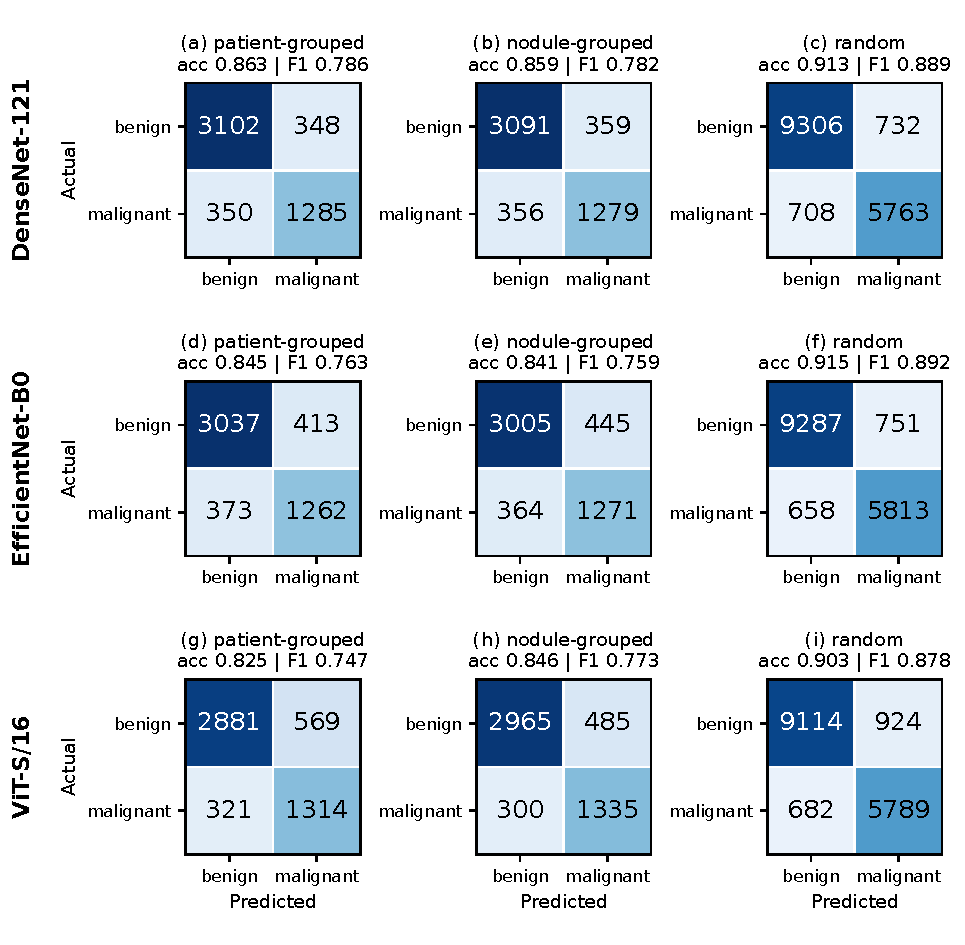
\includegraphics[width=0.92\textwidth]{confusion_matrices.pdf}
  \caption{Nodule-level confusion matrices at the $0.5$ threshold, summed over the 15 test folds of
  each arm (3 repeats $\times$ 5 folds); rows are architectures, columns are partition conditions,
  and accuracy and F1 for each panel are given above it. Cell shading is the within-panel proportion,
  so panels remain comparable despite differing totals. Within each repeat the five folds of the
  patient-grouped and nodule-grouped arms partition the cohort exactly, so each of the $1{,}695$
  nodules is scored once per repeat and three times in the totals shown ($3 \times 1{,}695 = 5{,}085$).
  In the random arm the test folds overlap by construction, so a nodule falls in $3.2$ of the five
  folds on average and its totals are correspondingly larger --- a faithful
  picture of what the leaky protocol produces, not a disjoint partition.
  Regenerated from the archived per-sample probabilities.}
  \label{fig:confusion}
\end{figure*}

\begin{figure*}[t]
  \centering
  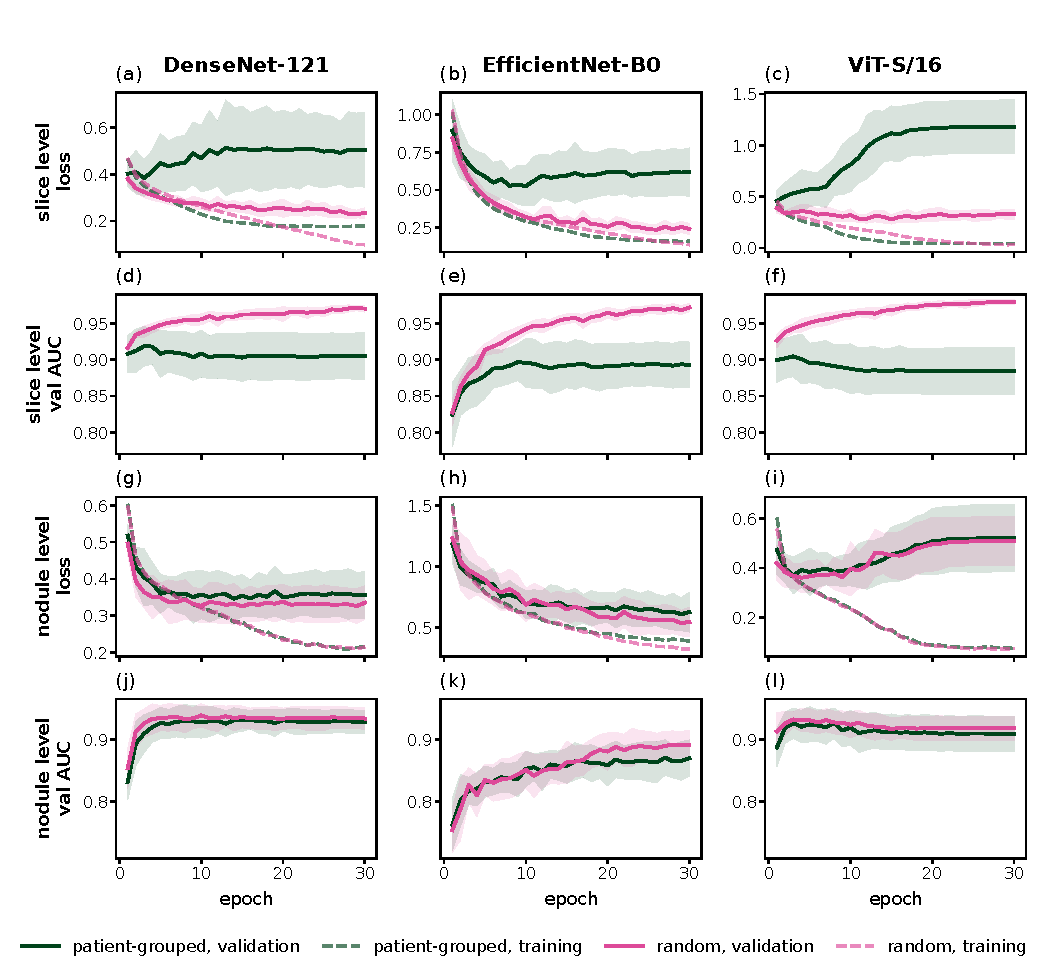
\includegraphics[width=\textwidth]{curves_slice-nodule.pdf}
  \caption{Learning curves for all three architectures, mean $\pm$ s.d.\ over the 15 runs of each
  arm; validation solid, training dashed. Columns are architectures; rows are the two quantities at
  each sample unit. \textbf{Slice level}, rows (a--c) loss and (d--f) validation AUC: under random
  partitioning (light magenta) the validation loss falls with the training loss and the validation AUC
  climbs to ${\approx}0.97$--$0.98$, the signature of memorizing a leaked split; under patient
  partitioning (dark green) the validation loss separates upward and the AUC plateaus near $0.905$
  (DenseNet-121), $0.893$ (EfficientNet-B0) and $0.885$ (ViT-S/16). \textbf{Nodule level}, rows
  (g--i) loss and (j--l) validation AUC: the same arms trained where within-nodule slice redundancy
  is absent by construction --- the two arms become nearly indistinguishable. The
  pattern replicates across all three backbones, including one with no convolutional inductive bias,
  so it is a property of the protocol rather than of a
  model. Within a row the three AUC panels share a $y$-range; the loss panels do not, because the
  backbones sit at different loss scales.
  \textbf{These are validation curves, and no value reported anywhere in this paper is computed from
  them.} They exist to select the checkpoint and to expose the mechanism; every metric in the Results
  and in Tables~\ref{tab:gap}--\ref{tab:routes} comes from the held-out test fold, as
  Section~\ref{sec:eval} states. The two are also different quantities: the validation AUC in rows
  (d--f) is per slice, and in rows (j--l) it is per nodule (one representative slice per nodule),
  whereas the AUCs quoted in the text are per-nodule test AUCs. Their closeness in the
  random arm is expected rather than coincidental, because a split that ignores the partition unit
  contaminates the validation fold in exactly the way it contaminates the test fold; in the
  patient-grouped arm, where both folds are clean, they differ.}
  \label{fig:curves}
\end{figure*}

Within-arm comparisons between architectures are informative about what leakage does to
benchmarking, and with three architectures the picture is more qualified than with two. For the two
convolutional backbones, McNemar's test separates them under patient partitioning ($b=319$, $c=231$,
$p=0.0002$) but not under random partitioning ($b=731$, $c=762$, $p=0.44$), where their absolute AUCs
converge to within $0.002$. The transformer does not follow that pattern: it remains distinguishable
from both CNNs in both arms: against DenseNet-121, $p = 2.5\times10^{-14}$ under patient
partitioning and $p = 7.1\times10^{-5}$ under random partitioning; against EfficientNet-B0,
$p = 1.3\times10^{-4}$ and $p = 2.4\times10^{-6}$.

Leakage therefore compresses the differences between models without abolishing them. The compression
is visible in the AUC spread, which narrows from $0.008$ across the three architectures under patient
partitioning to $0.005$ under random partitioning, and it is complete enough to erase a difference
that a clean protocol detects --- but only between the two architectures that were already the most
similar. We report this as the weaker claim it is: a leaked protocol raises every model towards a
ceiling set partly by memorization, which compresses the ranking, and it made two of our three
architectures statistically indistinguishable at the operating point when the clean protocol did not.
That is enough to make benchmark rankings obtained under leakage unreliable, and not enough to say
that architecture ceases to matter. It offers a partial explanation for a striking feature of the
literature --- reported performance on this benchmark is high and similar across widely different
architectures --- which our own three-architecture comparison supports for similar models and
qualifies for dissimilar ones.

\subsection{Learning dynamics}

Figure~\ref{fig:curves} shows the mechanism directly. Under random partitioning the validation loss
falls together with the training loss throughout training, because the validation fold is leaked in
exactly the way the test fold is; under patient partitioning the validation loss separates upward
from the training loss after a few epochs, the expected honest generalization gap. The selected
checkpoint reflects this: the best-validation-loss epoch averages $3.3$ (DenseNet-121), $10.9$
(EfficientNet-B0) and $2.6$ (ViT-S/16) in the patient arm against $23.4$, $26.3$ and $13.9$ in the
random arm.

\section{Discussion}
\textbf{Principal finding.} Holding cohort, labels, preprocessing, architecture, and training fixed
and varying only the partition unit, random partitioning inflated slice-level AUC by $+0.064$
(Nadeau--Bengio 95\% CI $+0.031$ to $+0.097$) for DenseNet-121, $+0.082$ ($+0.056$ to $+0.108$)
for EfficientNet-B0 and $+0.074$ ($+0.036$ to $+0.112$) for ViT-S/16, positive in 15 of 15 matched
folds for every architecture and unchanged when
both arms are re-scored on identical test rows. The magnitude should be read as specific to this
cohort, these architectures, and this protocol; what generalizes is the direction and the mechanism,
not the exact value.

\textbf{Mechanism.} Discrimination and calibration degrade to a comparable degree. Because a raw
comparison of an AUC gap against a log-loss gap is meaningless --- the two are not on a common scale
--- we express each gap in units of the between-fold standard deviation of the patient-arm value of
that same metric, a normalization applied identically to all three metrics. On that scale the gaps
are $2.7$ (AUC), $3.0$ (log-loss) and $3.0$ (Brier) fold-standard-deviations for DenseNet-121,
$4.0$, $3.1$ and $4.2$ for EfficientNet-B0, and $2.5$, $2.4$ and $2.9$ for ViT-S/16. Leakage
therefore does not act mainly on confidence while
sparing ranking: it moves discrimination and calibration by similar standardized amounts, and in two
of the three architectures the ranking metric moves at least as much as log-loss. We note this
explicitly because the unnormalized
numbers invite the opposite conclusion: dividing each gap by its own mean makes the calibration
effect look roughly six times larger, which is an artifact of AUC being bounded below by chance
rather than by zero. The learning curves make the
mechanism visible: under random partitioning the validation loss tracks training loss and keeps
falling (the leaked validation set is memorized alongside training), whereas under patient
partitioning validation loss diverges upward from training loss, the expected honest
generalization gap.

\textbf{The gap is not a test-set artifact.} Because the two arms have different test sets by
construction, a natural objection is that the gap reflects test-set composition rather than
leakage. We control for this by re-scoring both arms on the \emph{identical} rows (the same nodules
and slices present in both arms' test sets), holding composition, prevalence, size, and aggregation
depth fixed: the gap persists at $+0.064$ ($[+0.027, +0.101]$, DenseNet-121), $+0.080$
($[+0.047, +0.113]$, EfficientNet-B0) and $+0.075$ ($[+0.037, +0.113]$, ViT-S/16) at slice level,
15/15 folds in every case, and at the nodule-aggregated level
it is slightly \emph{larger} under the matched control than without it ($+0.058$, $+0.072$ and
$+0.066$). Composition therefore does not explain the effect.

\textbf{Architecture dependence.} The result was initially obtained on two convolutional backbones,
which left open whether it was a property of the partitioning protocol or of convolution. A
transformer could in principle exploit patient-level context that a convolutional inductive bias
does not, which would show up as a detectable patient route in ViT-S/16 and not in the two
convolutional backbones. That is
not what we observe. The combined gap replicates in the transformer at full strength ($+0.074$ in
AUC, 15/15 folds) and the patient route stays undetected there under the rule fixed in advance;
under the same non-interaction assumption that governs the other two architectures, the within-nodule
route again accounts for $81$--$87\%$ of the transformer's gap in log-loss and Brier. The finding
therefore holds
across two model families rather than within one, which is the stronger claim, and the null on the
patient route can no longer be attributed to convolutional inductive bias.

Two limits on that widening should be stated. Three architectures still sample the space of models
sparsely, and all three are ImageNet-pretrained and trained here with an identical recipe, so we
have varied the inductive bias but not the pretraining corpus or the optimization regime. And the
transformer, like the CNNs, was given no explicit patient-level input --- no identifier, no
acquisition metadata, no multi-slice context beyond a single image. What we have tested is whether
a model with global self-attention discovers patient identity from the image alone well enough to
change the measured gap. It does not appear to.

\textbf{Why the partition unit, and not stratification, governs the variance.} In grouped
cross-validation the fold-to-fold variance is driven by \emph{which patients} (hence which cases)
fall in a fold, not by the class proportion. We show this directly: the intra-class correlation of
the label within a patient is $0.339$ (design effect $1.44$; $74\%$ of patients carry only one label
class), so patients behave as partial label-blocks; an off-the-shelf stratified grouped split does
not reduce fold-prevalence spread here but very slightly increases it (nodule-level prevalence SD
$0.0328$ stratified against $0.0326$ unstratified, over 400 draws on the 740-patient pool), and a
near-perfect balancer buys essentially nothing: a swap-based
local search that drives the fold-prevalence SD from $0.0288$ to $0.00015$ --- a $192$-fold
improvement in precisely the quantity stratification optimizes --- changes the fold-to-fold SD of the
metrics by between $-7.3\%$ and $+0.7\%$, improving it slightly for the two convolutional backbones
and marginally worsening it for the transformer. (That projection holds the predictions fixed and re-partitions
them, so it isolates the fold-composition component of the variance, which is the only component a
balancer can remove; retraining under balanced folds would also perturb the predictions themselves
and is not captured.) The practical consequence is that
\emph{only $n$} (repeats $\times$ folds), not stratification, tightens the interval --- which is
why the design is repeated rather than stratified, and why single-split studies cannot quantify the
gap at all.

\textbf{Methodological implication.} Reporting slice-level performance without grouping does not
measure clinical generalization; it measures, in part, a model's ability to recognize \emph{lesions}
it has already seen, from adjacent and near-duplicate views of them. What we report is the size of
that inflation under a single, clean manipulation of the partition unit, on this cohort.

The practical recommendation follows from where the effect actually lives, and it is more specific
than the one usually given. \textbf{No study should partition below the nodule}: all slices of a lesion
must fall on the same side of the boundary. Under the assumption that the two routes do not
interact --- which three separately trained arms cannot test --- that single constraint captured
essentially all of the protection measurable in this cohort. Patient-level grouping is a strictly stronger condition --- it
implies nodule-level grouping --- and we did not detect that the additional constraint buys further
accuracy correction here; but it costs nothing to apply, it is the only choice that remains correct
if the two units diverge in a different cohort, and our interval leaves room for an effect we were
not powered to see. We therefore recommend patient-level grouping as the default, while noting that
the measurable damage in this benchmark comes from partitioning below the \emph{nodule}, and that a
study which groups by nodule but not by patient is far closer to an honest estimate than the
literature's framing would suggest. Independently of which unit is chosen, studies should state it
explicitly and release executable partition indices so the choice is auditable.

\textbf{Limitations.} The study uses 2D backbones on volumetric CT, mirroring the common practice
it audits; a 3D interaction is future work. Labels are radiologist-consensus rather than
histopathology; this label noise is identical across arms and so does not bias the paired contrast,
and we tested robustness to it on the high-agreement subcohort --- the nodules read by $\geq 3$
radiologists, where each median label rests on three or more independent readings rather than one. The gap
persists there: at slice level $+0.040$ (Nadeau--Bengio 95\% CI $[+0.021, +0.058]$) for DenseNet-121,
$+0.062$ ($[+0.030, +0.094]$) for EfficientNet-B0 and $+0.044$ ($[+0.021, +0.067]$) for ViT-S/16,
positive in 15 of 15 folds for all three, and
$+0.037$, $+0.061$ and $+0.046$ under the matched-rows control. Requiring three readers also removes the
nodules the radiologists disagreed about, and those are disproportionately benign, so the subcohort
is enriched for malignancy: the malignant share rises from $0.499$ to $0.638$ at slice level and from
$0.322$ to $0.489$ at nodule level. The point estimates there are smaller than in the principal
cohort, but that difference is \emph{not} attributable to label noise, because agreement and
prevalence moved together and log-loss and the Brier score are prevalence-sensitive; the analysis was
pre-specified as directional --- does the gap survive? --- and is led by AUC, the least
prevalence-sensitive of the three metrics.
The analysis is confined to LIDC-IDRI; external, multi-institutional validation is
valuable but out of scope for a methodological audit and is stated as future work. We validated the
pipeline on a 250-patient subset before scaling; those subset numbers are a pipeline check, not a
study result, and no value reported in this paper comes from that stage.

\textbf{Relation to prior audits.} The direction of the effect matches what audits in adjacent
medical-imaging domains have reported: correcting the evaluation protocol lowers the headline number~\vcite{wen2020,roberts2021}. We do not claim agreement in magnitude, because those audits differ from
this one in domain, task and the specific leakage they correct, and a numerical comparison across
them would not be meaningful.

\section{Conclusion}
Partitioning pulmonary-nodule data below the nodule inflates reported performance substantially. We
established this in a controlled experiment rather than by comparison with other studies, changing
only the unit at which folds are formed: slice-level partitioning raised AUC by $+0.064$, $+0.082$
and $+0.074$ across three architectures drawn from two model families, it did so in every one of 15
matched folds in each of them, and the
effect survived a control in which both conditions were re-scored on identical test rows, so it
cannot be explained by the two conditions having been tested on different cases.

Adding a third, nodule-grouped condition then localizes where that inflation comes from. Under the
assumption that the two routes do not interact, we did not detect a contribution from the patient
route in any architecture --- including a vision transformer, so the null cannot be attributed to
convolutional inductive bias --- whereas within-nodule slice redundancy accounted for $81$--$98\%$ of
the gap in log-loss and in Brier. We make no such attribution for AUC, which is a rank statistic and
does not decompose over the samples a route acts on. Grouping folds at
the nodule therefore captured essentially all of the protection available in this cohort. Patient-level
grouping did not add a detectable further margin, but it remains the safer default, both because it
guarantees the same protection and because the two units can diverge in cohorts other than this one.

The operative recommendation is consequently narrower and firmer than the usual advice. No study
should partition below the nodule; every study should state its partition unit explicitly, since a
large part of the literature currently does not; and every study should release executable partition
indices, so that the choice can be audited by a reader rather than taken on trust.

\section*{Data and Code Availability}
All code, partition indices and per-sample predictions supporting this study are openly available at
\url{https://github.com/nykemariotto/nodule-partition-leakage}. Every table and figure in this paper
can be regenerated from that repository without a GPU and without retraining: \texttt{outputs/splits/}
holds the exact fold assignments, one table per fold, so the partitions can be reconstructed rather
than taken on trust; \texttt{outputs/probs/} holds the predicted probability of every image in every
run, which is what makes the reported statistics recomputable; and \texttt{outputs/results/} holds
the derived tables, including the complete per-model metrics and the confusion-matrix counts, each
produced by the released code rather than transcribed. Cohort construction is documented in
\texttt{dataset\_accounting.md}, and \texttt{partition\_unit\_survey.md} records, for each study
surveyed in Related Work, the partition unit it declares and the sentence we classified it on. The underlying images are not redistributed here: LIDC-IDRI is
publicly available from The Cancer Imaging Archive under its own terms, and the released metadata
identify the exact scans, nodules and slices used.


\section*{Acknowledgment}
The authors specified the experimental design and every methodological decision in this work,
reviewed and verified all AI-assisted code and text, and independently confirmed each reported
result against the artifacts produced by the released code. In carrying out that work the authors
used a large language model (Claude, Anthropic), operated through the agentic coding assistant
Claude Code, and disclose its use as follows. (i) The experimental-pipeline code (metadata
construction, preprocessing, partition-index generation, model training, and evaluation) was
implemented with the tool's assistance and reviewed by the authors. (ii) The statistical-analysis
and figure-generation code was implemented and reviewed in the same way. (iii) Text in the
Introduction, Related Work, Methods, and Discussion, and in the response to reviewers, was drafted
with the tool's assistance and revised by the authors. (iv) The tool assisted in checking the
bibliographic details of the cited references against primary sources. (v) It also read the methods
sections of the studies surveyed in Related Work and extracted from each the partition unit that
study declares; every study reported in that survey is cited, and the sentence on which each was
classified is quoted verbatim in the released survey table
(\texttt{partition\_unit\_survey.md}), so the classification can be checked against its source
rather than taken on trust, and the authors confirmed each extraction against the source study.

Every figure in this manuscript, including the method schematic, is a deterministic rendering
produced by the released plotting scripts (matplotlib) run on real artifacts; no generative
image- or figure-synthesis system was used to create any figure or image in this work. The
scientific content, methodological decisions, data, results, interpretations, and conclusions are
the authors' own; the authors take full responsibility for the integrity and accuracy of the
manuscript. No AI system is an author of this work.

\section*{Author Contributions}
N. Mariotto: conceptualization, investigation, methodology, validation, visualization, formal analysis, data curation, writing---original draft, writing---review and editing, and supervision. J. G. Ferreira: investigation, methodology, and data curation. J. R. Almeida de Andrade: data curation, methodology, and investigation. J. V. Carneiro Faria: methodology, data curation, and investigation. A. F. Fattori Alves: project administration, supervision, funding acquisition, formal analysis, data curation, writing---original draft, and writing---review and editing.




% Generated by IEEEtran.bst, version: 1.14 (2015/08/26)
\begin{thebibliography}{10}
\providecommand{\url}[1]{#1}
\csname url@samestyle\endcsname
\providecommand{\newblock}{\relax}
\providecommand{\bibinfo}[2]{#2}
\providecommand{\BIBentrySTDinterwordspacing}{\spaceskip=0pt\relax}
\providecommand{\BIBentryALTinterwordstretchfactor}{4}
\providecommand{\BIBentryALTinterwordspacing}{\spaceskip=\fontdimen2\font plus
\BIBentryALTinterwordstretchfactor\fontdimen3\font minus \fontdimen4\font\relax}
\providecommand{\BIBforeignlanguage}[2]{{%
\expandafter\ifx\csname l@#1\endcsname\relax
\typeout{** WARNING: IEEEtran.bst: No hyphenation pattern has been}%
\typeout{** loaded for the language `#1'. Using the pattern for}%
\typeout{** the default language instead.}%
\else
\language=\csname l@#1\endcsname
\fi
#2}}
\providecommand{\BIBdecl}{\relax}
\BIBdecl

\bibitem{bray2024}
F.~Bray, M.~Laversanne, H.~Sung, J.~Ferlay, R.~L. Siegel, I.~Soerjomataram, and A.~Jemal, ``Global cancer statistics 2022: {GLOBOCAN} estimates of incidence and mortality worldwide for 36 cancers in 185 countries,'' \emph{CA Cancer J. Clin.}, vol.~74, no.~3, pp. 229--263, May–Jun. 2024, doi: 10.3322/caac.21834.

\bibitem{aberle2011}
{National Lung Screening Trial Research Team}, D.~R. Aberle, A.~M. Adams, C.~D. Berg, W.~C. Black, J.~D. Clapp, R.~M. Fagerstrom, I.~F. Gareen, C.~Gatsonis, P.~M. Marcus, and J.~D. Sicks, ``Reduced lung-cancer mortality with low-dose computed tomographic screening,'' \emph{N. Engl. J. Med.}, vol. 365, no.~5, pp. 395--409, Aug. 2011, doi: 10.1056/NEJMoa1102873.

\bibitem{macmahon2017}
H.~MacMahon, D.~P. Naidich, J.~M. Goo, K.~S. Lee, A.~N.~C. Leung, J.~R. Mayo, A.~C. Mehta, Y.~Ohno, C.~A. Powell, M.~Prokop, G.~D. Rubin, C.~M. Schaefer-Prokop, W.~D. Travis, P.~E. Van~Schil, and A.~A. Bankier, ``Guidelines for management of incidental pulmonary nodules detected on {CT} images: From the {Fleischner Society} 2017,'' \emph{Radiology}, vol. 284, no.~1, pp. 228--243, Jul. 2017, doi: 10.1148/radiol.2017161659.

\bibitem{armato2011}
S.~G. {Armato III} \emph{et~al.}, ``The lung image database consortium ({LIDC}) and image database resource initiative ({IDRI}): A completed reference database of lung nodules on {CT} scans,'' \emph{Medical Physics}, vol.~38, no.~2, pp. 915--931, Feb. 2011, doi: 10.1118/1.3528204.

\bibitem{wen2020}
J.~Wen, E.~Thibeau-Sutre, M.~Diaz-Melo, J.~Samper-Gonz{\'a}lez, A.~Routier, S.~Bottani, D.~Dormont, S.~Durrleman, N.~Burgos, O.~Colliot, {Alzheimer's Disease Neuroimaging Initiative}, and {Australian Imaging Biomarkers and Lifestyle flagship study of ageing}, ``Convolutional neural networks for classification of {A}lzheimer's disease: Overview and reproducible evaluation,'' \emph{Medical Image Analysis}, vol.~63, p. 101694, Jul. 2020, doi: 10.1016/j.media.2020.101694.

\bibitem{roberts2021}
M.~Roberts, D.~Driggs, M.~Thorpe, J.~Gilbey, M.~Yeung, S.~Ursprung, A.~I. Aviles-Rivero, C.~Etmann, C.~McCague, L.~Beer, J.~R. Weir-McCall, Z.~Teng, E.~Gkrania-Klotsas, {AIX-COVNET}, J.~H.~F. Rudd, E.~Sala, and C.-B. Sch{\"o}nlieb, ``Common pitfalls and recommendations for using machine learning to detect and prognosticate for {COVID}-19 using chest radiographs and {CT} scans,'' \emph{Nature Machine Intelligence}, vol.~3, no.~3, pp. 199--217, 2021, doi: 10.1038/s42256-021-00307-0.

\bibitem{jin2025}
H.~Jin, C.~Yu, J.~Zhang, R.~Zheng, Y.~Fu, and Y.~Zhao, ``Multitask {S}win {T}ransformer for classification and characterization of pulmonary nodules in {CT} images,'' \emph{Quantitative Imaging in Medicine and Surgery}, vol.~15, no.~3, pp. 1845--1861, Mar. 2025, doi: 10.21037/qims-24-1619.

\bibitem{thakur2026}
N.~Thakur, P.~Chouksey, A.~Sharma, M.~Chopra, P.~Sadotra, and S.~Kumar, ``Binary classification of lung cancer using vision transformer models on {CT} images,'' \emph{Discover Computing}, vol.~29, no.~1, 2026, doi: 10.1007/s10791-026-09931-z.

\bibitem{alshabi2019gated}
M.~Al-Shabi, H.~K. Lee, and M.~Tan, ``Gated-dilated networks for lung nodule classification in {CT} scans,'' \emph{IEEE Access}, vol.~7, pp. 178\,827--178\,838, 2019, doi: 10.1109/ACCESS.2019.2958663.

\bibitem{procan2021}
M.~Al-Shabi, K.~Shak, and M.~Tan, ``{ProCAN}: Progressive growing channel attentive non-local network for lung nodule classification,'' \emph{Pattern Recognit.}, vol. 122, p. 108309, 2022, doi: 10.1016/j.patcog.2021.108309.

\bibitem{xiao2020ens}
N.~Xiao, Y.~Qiang, M.~Bilal~Zia, S.~Wang, and J.~Lian, ``Ensemble classification for predicting the malignancy level of pulmonary nodules on chest computed tomography images,'' \emph{Oncol. Lett.}, vol.~20, no.~1, pp. 401--408, Jul. 2020, doi: 10.3892/ol.2020.11576.

\bibitem{contrastdiag2024}
\BIBentryALTinterwordspacing
C.~Wang, Y.~Yi, Y.~Wang, C.~Zhang, Y.~Liu, K.~Mori, M.~Yuan, and G.~Yang, ``{ContrastDiagnosis}: Enhancing interpretability in lung nodule diagnosis using contrastive learning,'' 2024, arXiv:2403.05280. [Online]. Available: \url{https://arxiv.org/abs/2403.05280}
\BIBentrySTDinterwordspacing

\bibitem{lmlcc2025}
\BIBentryALTinterwordspacing
T.~B. Mamun, A.~Madhuri, N.~Sobir, and T.~Hasan, ``{LMLCC-Net}: A semi-supervised deep learning model for lung nodule malignancy prediction from {CT} scans,'' 2025, arXiv:2505.06370. [Online]. Available: \url{https://arxiv.org/abs/2505.06370}
\BIBentrySTDinterwordspacing

\bibitem{alshabi2019lg}
M.~Al-Shabi, B.~L. Lan, W.~Y. Chan, K.-H. Ng, and M.~Tan, ``Lung nodule classification using deep local--global networks,'' \emph{Int. J. Comput. Assist. Radiol. Surg.}, vol.~14, no.~10, pp. 1815--1819, Oct. 2019, doi: 10.1007/s11548-019-01981-7.

\bibitem{attnpyramid2024}
H.~Wang, H.~Zhu, L.~Ding, and K.~Yang, ``Attention pyramid pooling network for artificial diagnosis on pulmonary nodules,'' \emph{PLoS ONE}, vol.~19, no.~5, p. e0302641, May 2024, doi: 10.1371/journal.pone.0302641.

\bibitem{pitfalls2021}
V.~Baltatzis, K.-M. Bintsi, L.~{Le Folgoc}, O.~E. Martinez~Manzanera, S.~Ellis, A.~Nair, S.~Desai, B.~Glocker, and J.~A. Schnabel, ``The pitfalls of sample selection: A case study on lung nodule classification,'' in \emph{Predictive Intelligence in Medicine ({PRIME} 2021)}, ser. Lecture Notes in Computer Science, vol. 12928.\hskip 1em plus 0.5em minus 0.4em\relax Springer, 2021, pp. 201--211, doi: 10.1007/978-3-030-87602-9\_19.

\bibitem{kaufman2012}
S.~Kaufman, S.~Rosset, C.~Perlich, and O.~Stitelman, ``Leakage in data mining: Formulation, detection, and avoidance,'' \emph{ACM Transactions on Knowledge Discovery from Data}, vol.~6, no.~4, pp. 1--21, 2012, doi: 10.1145/2382577.2382579.

\bibitem{mcn2020}
P.~Afshar, A.~Oikonomou, F.~Naderkhani, P.~N. Tyrrell, K.~N. Plataniotis, K.~Farahani, and A.~Mohammadi, ``{3D-MCN}: A {3D} multi-scale capsule network for lung nodule malignancy prediction,'' \emph{Sci. Rep.}, vol.~10, p. 7948, May 2020, doi: 10.1038/s41598-020-64824-5.

\bibitem{cmixnet2019}
N.~Nasrullah, J.~Sang, M.~S. Alam, M.~Mateen, B.~Cai, and H.~Hu, ``Automated lung nodule detection and classification using deep learning combined with multiple strategies,'' \emph{Sensors}, vol.~19, no.~17, p. 3722, Aug. 2019, doi: 10.3390/s19173722.

\bibitem{mase2025}
\BIBentryALTinterwordspacing
U.~Saha and S.~Prakash, ``Multi-attention stacked ensemble for lung cancer detection in {CT} scans,'' 2025, arXiv:2507.20221. [Online]. Available: \url{https://arxiv.org/abs/2507.20221}
\BIBentrySTDinterwordspacing

\bibitem{pedrosa2021}
J.~Pedrosa, G.~Aresta, C.~Ferreira, G.~Atwal, H.~A. Phoulady, X.~Chen, R.~Chen, J.~Li, L.~Wang, A.~Galdran, H.~Bouchachia, K.~C. Kaluva, K.~Vaidhya, A.~Chunduru, S.~Tarai, S.~P.~P. Nadimpalli, S.~Vaidya, I.~Kim, A.~Rassadin, Z.~Tian, Z.~Sun, Y.~Jia, X.~Men, I.~Ramos, A.~Cunha, and A.~Campilho, ``{LNDb} challenge on automatic lung cancer patient management,'' \emph{Medical Image Analysis}, vol.~70, p. 102027, May 2021, doi: 10.1016/j.media.2021.102027.

\bibitem{hancock2016}
M.~C. Hancock and J.~F. Magnan, ``Lung nodule malignancy classification using only radiologist-quantified image features as inputs to statistical learning algorithms: probing the {Lung Image Database Consortium} dataset with two statistical learning methods,'' \emph{Journal of Medical Imaging}, vol.~3, no.~4, p. 044504, Oct. 2016, describes the pylidc library in its Appendix; \url{https://pylidc.github.io/}, doi: 10.1117/1.JMI.3.4.044504.

\bibitem{kubota2011}
T.~Kubota, A.~K. Jerebko, M.~Dewan, M.~Salganicoff, and A.~Krishnan, ``Segmentation of pulmonary nodules of various densities with morphological approaches and convexity models,'' \emph{Medical Image Analysis}, vol.~15, no.~1, pp. 133--154, Feb. 2011, doi: 10.1016/j.media.2010.08.005.

\bibitem{huang2017densenet}
G.~Huang, Z.~Liu, L.~Van Der~Maaten, and K.~Q. Weinberger, ``Densely connected convolutional networks,'' in \emph{2017 {IEEE} Conference on Computer Vision and Pattern Recognition ({CVPR})}.\hskip 1em plus 0.5em minus 0.4em\relax IEEE, 2017, pp. 2261--2269, doi: 10.1109/CVPR.2017.243.

\bibitem{tan2019efficientnet}
M.~Tan and Q.~Le, ``{EfficientNet}: Rethinking model scaling for convolutional neural networks,'' in \emph{Proceedings of the 36th International Conference on Machine Learning}, ser. Proceedings of Machine Learning Research, vol.~97.\hskip 1em plus 0.5em minus 0.4em\relax PMLR, 2019, pp. 6105--6114.

\bibitem{dosovitskiy2021vit}
A.~Dosovitskiy, L.~Beyer, A.~Kolesnikov, D.~Weissenborn, X.~Zhai, T.~Unterthiner, M.~Dehghani, M.~Minderer, G.~Heigold, S.~Gelly, J.~Uszkoreit, and N.~Houlsby, ``An image is worth 16x16 words: Transformers for image recognition at scale,'' in \emph{International Conference on Learning Representations ({ICLR})}, 2021.

\bibitem{nadeau2003}
C.~Nadeau and Y.~Bengio, ``Inference for the generalization error,'' \emph{Machine Learning}, vol.~52, no.~3, pp. 239--281, 2003, doi: 10.1023/A:1024068626366.

\end{thebibliography}

\begin{IEEEbiographynophoto}{Nycolas Mariotto}
received the B.Sc. degree in medical physics and the M.Sc. degree in biomolecular and pharmacological sciences from S\~ao Paulo State University (UNESP), Botucatu, Brazil, where he is currently pursuing the Ph.D. degree in biomolecular and pharmacological sciences. His research develops and applies convolutional neural networks, foundation models (SAM, SAMed), and other advanced artificial intelligence architectures to the multiscale processing of medical and biomedical images, covering detection, automated segmentation, and classification of pathology across optical and transmission electron microscopy, computed tomography, and magnetic resonance imaging. He works on quantitative image analysis, radiomic feature extraction (shape, texture, volume, and density), computational modeling, and integrated pipelines for diagnostic support, as well as on diffusion-based generative models (DiffBoost, MedDiffusion, CellDiffusion) for biomedical data synthesis, self-supervised learning, and interpretability methods (SHAP, LASSO) that turn quantitative measurements into explainable findings. His interests include computer vision for healthcare, transformer architectures (SwinUNETR, nnFormer++, TransUNet), segmentation of cellular and ultrastructural targets such as mitochondria, organelles, pulmonary nodules, and brain tumors, the integration of artificial intelligence tools into clinical systems, and the development of quantitative biomarkers for biophysical, pharmacological, and diagnostic applications.
\end{IEEEbiographynophoto}
\begin{IEEEbiographynophoto}{Jadson Gabriel Ferreira}
received the B.Sc. degree in medical physics from S\~ao Paulo State University (UNESP), Botucatu, Brazil, where he is currently pursuing the M.Sc. degree in biometry. His current research is in artificial intelligence, developing quantum machine learning models for the diagnosis of brain tumors from magnetic resonance imaging. He has experience with deep learning and with convolutional and quantum convolutional neural networks applied to medical image processing, including pulmonary nodule classification. During his undergraduate studies he served as a teaching assistant in quantum mechanics, solid-state physics, and modern physics, and took part in science-outreach projects. He has complementary training in Python and quantum computing.
\end{IEEEbiographynophoto}
\begin{IEEEbiographynophoto}{Jo\~ao Rafael Almeida de Andrade}
received the B.Sc. degree in medical physics from S\~ao Paulo State University (UNESP), Botucatu, Brazil. His research interests include data curation and methodological aspects of deep learning applied to medical imaging.
\end{IEEEbiographynophoto}
\begin{IEEEbiographynophoto}{Jo\~ao Victor Carneiro Faria}
received the B.Sc. degree in medical physics and the M.Sc. degree in biological sciences (pharmacology) from S\~ao Paulo State University (UNESP), Botucatu, Brazil, where he is currently pursuing the Ph.D. degree in biomolecular and pharmacological sciences. His doctoral project develops artificial intelligence methods for opportunistic diagnosis, combining automated detection of incidental findings in imaging examinations using convolutional neural networks with the analysis of structured and unstructured clinical data. His current research concerns the curation, harmonization, and quality control of multicentric medical imaging and clinical datasets, addressing intensity normalization, domain adaptation, and the standardization of clinical variables across institutions. He also works on machine learning for clinical outcome prediction, applying gradient boosting methods together with patient stratification and SHAP-based interpretability to predict hospital length of stay across patient subgroups. His research interests include medical image harmonization, opportunistic screening, CNN-based medical image analysis, clinical predictive analytics, patient stratification, and interpretable machine learning for healthcare.
\end{IEEEbiographynophoto}
\begin{IEEEbiographynophoto}{Allan Felipe Fattori Alves}
received the B.Sc. degree in medical physics and the M.Sc. degree in general and applied biology, in the area of radiodiagnosis, from S\~ao Paulo State University (UNESP), Botucatu, Brazil, and the Ph.D. degree under a cotutelle agreement between the Pharmacology and Biotechnology program at UNESP, Botucatu, and the ``Sant\'e, Sciences Biologiques et Chimie du Vivant'' program at the University of Orl\'eans, France. He is currently an Assistant Professor with the Department of Biophysics and Pharmacology, Institute of Biosciences, S\~ao Paulo State University (UNESP), Botucatu, Brazil, and a researcher at Instituto Hardware BR (HBR), where he works on the Hardware Avan\c{c}ado para Imagens M\'edicas (HAPI) project, which developed an X-ray computed tomography scanner. He serves as treasurer on the 2024--2025 board of the Brazilian Association of Medical Physics. His main interests are medical signal and image processing, the development of computational algorithms and of tools to support medical diagnosis, applications of artificial intelligence, and hardware development for medicine.
\end{IEEEbiographynophoto}

\EOD

\end{document}
